\tikzset{every picture/.style={line width=0.75pt}} %set default line width to 0.75pt        

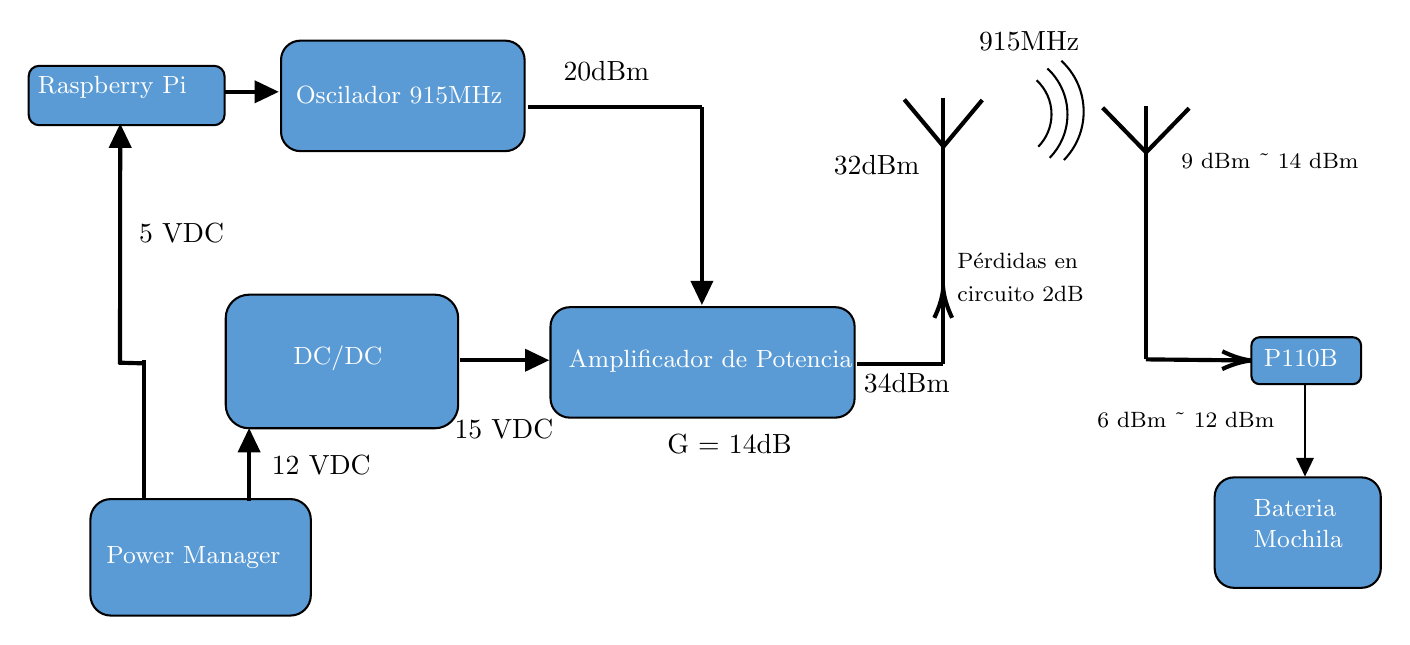
\begin{tikzpicture}[x=0.75pt,y=0.75pt,yscale=-1,xscale=1]
%uncomment if require: \path (0,417); %set diagram left start at 0, and has height of 417

%Flowchart: Alternative Process [id:dp5901024681209728] 
\draw  [color={rgb, 255:red, 0; green, 0; blue, 0 }  ,draw opacity=1 ][fill={rgb, 255:red, 91; green, 155; blue, 213 }  ,fill opacity=1 ] (3.83,27.9) .. controls (3.83,25.14) and (6.07,22.9) .. (8.84,22.9) -- (93.17,22.9) .. controls (95.94,22.9) and (98.18,25.14) .. (98.18,27.9) -- (98.18,46.49) .. controls (98.18,49.25) and (95.94,51.49) .. (93.17,51.49) -- (8.84,51.49) .. controls (6.07,51.49) and (3.83,49.25) .. (3.83,46.49) -- cycle ;
%Straight Lines [id:da5704480834754568] 
\draw [line width=1.5]    (47.83,166.5) -- (47.91,54.79) ;
\draw [shift={(47.92,50.79)}, rotate = 450.04] [fill={rgb, 255:red, 0; green, 0; blue, 0 }  ][line width=0.08]  [draw opacity=0] (11.61,-5.58) -- (0,0) -- (11.61,5.58) -- cycle    ;
%Straight Lines [id:da41020422247527444] 
\draw [line width=1.5]    (98.03,35.41) -- (120.25,35.41) ;
\draw [shift={(124.25,35.41)}, rotate = 180] [fill={rgb, 255:red, 0; green, 0; blue, 0 }  ][line width=0.08]  [draw opacity=0] (11.61,-5.58) -- (0,0) -- (11.61,5.58) -- cycle    ;
%Flowchart: Alternative Process [id:dp9678129498459402] 
\draw  [color={rgb, 255:red, 0; green, 0; blue, 0 }  ,draw opacity=1 ][fill={rgb, 255:red, 91; green, 155; blue, 213 }  ,fill opacity=1 ] (125.4,20.07) .. controls (125.4,14.93) and (129.57,10.76) .. (134.71,10.76) -- (233.44,10.76) .. controls (238.58,10.76) and (242.75,14.93) .. (242.75,20.07) -- (242.75,54.66) .. controls (242.75,59.81) and (238.58,63.98) .. (233.44,63.98) -- (134.71,63.98) .. controls (129.57,63.98) and (125.4,59.81) .. (125.4,54.66) -- cycle ;
%Flowchart: Alternative Process [id:dp03056880673326523] 
\draw  [color={rgb, 255:red, 0; green, 0; blue, 0 }  ,draw opacity=1 ][fill={rgb, 255:red, 91; green, 155; blue, 213 }  ,fill opacity=1 ] (33.56,241.45) .. controls (33.56,236.03) and (37.96,231.63) .. (43.38,231.63) -- (129.93,231.63) .. controls (135.35,231.63) and (139.75,236.03) .. (139.75,241.45) -- (139.75,277.93) .. controls (139.75,283.35) and (135.35,287.75) .. (129.93,287.75) -- (43.38,287.75) .. controls (37.96,287.75) and (33.56,283.35) .. (33.56,277.93) -- cycle ;
%Flowchart: Alternative Process [id:dp843232670273814] 
\draw  [color={rgb, 255:red, 0; green, 0; blue, 0 }  ,draw opacity=1 ][fill={rgb, 255:red, 91; green, 155; blue, 213 }  ,fill opacity=1 ] (98.76,144.42) .. controls (98.76,138.19) and (103.8,133.15) .. (110.02,133.15) -- (199.48,133.15) .. controls (205.7,133.15) and (210.74,138.19) .. (210.74,144.42) -- (210.74,186.26) .. controls (210.74,192.48) and (205.7,197.52) .. (199.48,197.52) -- (110.02,197.52) .. controls (103.8,197.52) and (98.76,192.48) .. (98.76,186.26) -- cycle ;
%Flowchart: Alternative Process [id:dp2196391995059177] 
\draw  [color={rgb, 255:red, 0; green, 0; blue, 0 }  ,draw opacity=1 ][fill={rgb, 255:red, 91; green, 155; blue, 213 }  ,fill opacity=1 ] (255.23,148.49) .. controls (255.23,143.35) and (259.4,139.18) .. (264.54,139.18) -- (392.44,139.18) .. controls (397.58,139.18) and (401.75,143.35) .. (401.75,148.49) -- (401.75,183.08) .. controls (401.75,188.22) and (397.58,192.39) .. (392.44,192.39) -- (264.54,192.39) .. controls (259.4,192.39) and (255.23,188.22) .. (255.23,183.08) -- cycle ;
%Straight Lines [id:da8714121235465184] 
\draw [line width=1.5]    (59.5,231.17) -- (59.5,164.83) ;
%Straight Lines [id:da4234181334294336] 
\draw [line width=1.5]    (110.02,232.4) -- (110.02,201.52) ;
\draw [shift={(110.02,197.52)}, rotate = 450] [fill={rgb, 255:red, 0; green, 0; blue, 0 }  ][line width=0.08]  [draw opacity=0] (11.61,-5.58) -- (0,0) -- (11.61,5.58) -- cycle    ;
%Straight Lines [id:da32310599172032184] 
\draw [line width=1.5]    (211.59,164.74) -- (250.55,164.74) ;
\draw [shift={(254.55,164.74)}, rotate = 180] [fill={rgb, 255:red, 0; green, 0; blue, 0 }  ][line width=0.08]  [draw opacity=0] (11.61,-5.58) -- (0,0) -- (11.61,5.58) -- cycle    ;
%Straight Lines [id:da10232257644239184] 
\draw [line width=1.5]    (328.18,42.66) -- (328.18,134.07) ;
\draw [shift={(328.18,138.07)}, rotate = 270] [fill={rgb, 255:red, 0; green, 0; blue, 0 }  ][line width=0.08]  [draw opacity=0] (11.61,-5.58) -- (0,0) -- (11.61,5.58) -- cycle    ;
%Straight Lines [id:da7533713101555997] 
\draw [line width=1.5]    (244.32,42.66) -- (328.18,42.66) ;
%Straight Lines [id:da7648549186794515] 
\draw [line width=1.5]    (402.74,166.51) -- (444.43,166.51) ;
%Straight Lines [id:da35576594493962777] 
\draw [line width=1.5]    (444.43,166.51) -- (444.43,133.09) ;
\draw [shift={(444.43,130.09)}, rotate = 450] [color={rgb, 255:red, 0; green, 0; blue, 0 }  ][line width=1.5]    (14.21,-4.28) .. controls (9.04,-1.82) and (4.3,-0.39) .. (0,0) .. controls (4.3,0.39) and (9.04,1.82) .. (14.21,4.28)   ;
%Straight Lines [id:da02646954268865498] 
\draw [line width=1.5]    (444.43,38.25) -- (444.43,130.09) ;
%Straight Lines [id:da4914114624712449] 
\draw [line width=1.5]    (425.69,39.12) -- (444.58,61.75) ;
%Straight Lines [id:da9035567772895365] 
\draw [line width=1.5]    (444.58,61.75) -- (463.25,39.38) ;

%Shape: Arc [id:dp5933295871897399] 
\draw  [draw opacity=0] (494.61,24.16) .. controls (500.61,29.68) and (504.35,37.62) .. (504.3,46.42) .. controls (504.25,54.52) and (500.99,61.86) .. (495.73,67.23) -- (474.3,46.23) -- cycle ; \draw   (494.61,24.16) .. controls (500.61,29.68) and (504.35,37.62) .. (504.3,46.42) .. controls (504.25,54.52) and (500.99,61.86) .. (495.73,67.23) ;
%Shape: Arc [id:dp846123263641188] 
\draw  [draw opacity=0] (489.41,29.82) .. controls (493.87,33.93) and (496.65,39.83) .. (496.61,46.37) .. controls (496.57,52.4) and (494.15,57.85) .. (490.24,61.84) -- (474.3,46.23) -- cycle ; \draw   (489.41,29.82) .. controls (493.87,33.93) and (496.65,39.83) .. (496.61,46.37) .. controls (496.57,52.4) and (494.15,57.85) .. (490.24,61.84) ;
%Shape: Arc [id:dp3021222167053754] 
\draw  [draw opacity=0] (501.35,20.47) .. controls (508.01,26.6) and (512.16,35.4) .. (512.1,45.17) .. controls (512.04,54.16) and (508.42,62.3) .. (502.59,68.26) -- (478.81,44.96) -- cycle ; \draw   (501.35,20.47) .. controls (508.01,26.6) and (512.16,35.4) .. (512.1,45.17) .. controls (512.04,54.16) and (508.42,62.3) .. (502.59,68.26) ;
%Straight Lines [id:da33760072063062574] 
\draw [line width=1.5]    (590.08,164.83) -- (542.04,164.32) ;
\draw [shift={(593.08,164.87)}, rotate = 180.61] [color={rgb, 255:red, 0; green, 0; blue, 0 }  ][line width=1.5]    (14.21,-4.28) .. controls (9.04,-1.82) and (4.3,-0.39) .. (0,0) .. controls (4.3,0.39) and (9.04,1.82) .. (14.21,4.28)   ;
%Straight Lines [id:da3851997872773145] 
\draw [line width=1.5]    (542.04,164.32) -- (542.04,129.66) ;
%Straight Lines [id:da9393977842068026] 
\draw [line width=1.5]    (542.04,42.25) -- (542.04,129.66) ;
%Straight Lines [id:da6609719078207286] 
\draw [line width=1.5]    (521.25,43.08) -- (542.2,64.62) ;
%Straight Lines [id:da1212283700039476] 
\draw [line width=1.5]    (542.2,64.62) -- (562.9,43.32) ;
%Flowchart: Alternative Process [id:dp07927580495302378] 
\draw  [color={rgb, 255:red, 0; green, 0; blue, 0 }  ,draw opacity=1 ][fill={rgb, 255:red, 91; green, 155; blue, 213 }  ,fill opacity=1 ] (592.93,157.61) .. controls (592.93,155.43) and (594.69,153.66) .. (596.88,153.66) -- (641.8,153.66) .. controls (643.98,153.66) and (645.75,155.43) .. (645.75,157.61) -- (645.75,172.3) .. controls (645.75,174.48) and (643.98,176.25) .. (641.8,176.25) -- (596.88,176.25) .. controls (594.69,176.25) and (592.93,174.48) .. (592.93,172.3) -- cycle ;
%Straight Lines [id:da9089373110098913] 
\draw [line width=1.5]    (47.03,165.9) -- (58.7,166.23) ;
%Flowchart: Alternative Process [id:dp4035191156494293] 
\draw  [color={rgb, 255:red, 0; green, 0; blue, 0 }  ,draw opacity=1 ][fill={rgb, 255:red, 91; green, 155; blue, 213 }  ,fill opacity=1 ] (575.23,230.49) .. controls (575.23,225.35) and (579.4,221.18) .. (584.54,221.18) -- (645.94,221.18) .. controls (651.08,221.18) and (655.25,225.35) .. (655.25,230.49) -- (655.25,265.08) .. controls (655.25,270.22) and (651.08,274.39) .. (645.94,274.39) -- (584.54,274.39) .. controls (579.4,274.39) and (575.23,270.22) .. (575.23,265.08) -- cycle ;
%Straight Lines [id:da744994327328814] 
\draw    (618.75,176.75) -- (618.75,217.75) ;
\draw [shift={(618.75,220.75)}, rotate = 270] [fill={rgb, 255:red, 0; green, 0; blue, 0 }  ][line width=0.08]  [draw opacity=0] (8.93,-4.29) -- (0,0) -- (8.93,4.29) -- cycle    ;

% Text Node
\draw (130.99,31.44) node [anchor=north west][inner sep=0.75pt]  [font=\small,color={rgb, 255:red, 255; green, 255; blue, 255 }  ,opacity=1 ] [align=left] {{\small Oscilador 915MHz}};
% Text Node
\draw (39.8,252.91) node [anchor=north west][inner sep=0.75pt]  [font=\small,color={rgb, 255:red, 255; green, 255; blue, 255 }  ,opacity=1 ] [align=left] {{\small Power Manager}};
% Text Node
\draw (129.87,156.47) node [anchor=north west][inner sep=0.75pt]  [font=\small,color={rgb, 255:red, 255; green, 255; blue, 255 }  ,opacity=1 ] [align=left] {{\small DC/DC}};
% Text Node
\draw (262.52,158.45) node [anchor=north west][inner sep=0.75pt]  [font=\small,color={rgb, 255:red, 255; green, 255; blue, 255 }  ,opacity=1 ] [align=left] {{\small Amplificador de Potencia}};
% Text Node
\draw (597.42,158.03) node [anchor=north west][inner sep=0.75pt]  [font=\small,color={rgb, 255:red, 255; green, 255; blue, 255 }  ,opacity=1 ] [align=left] {P110B};
% Text Node
\draw (6.77,26.28) node [anchor=north west][inner sep=0.75pt]  [color={rgb, 255:red, 255; green, 255; blue, 255 }  ,opacity=1 ] [align=left] {{\small Raspberry Pi}};
% Text Node
\draw (592.52,230.45) node [anchor=north west][inner sep=0.75pt]  [font=\small,color={rgb, 255:red, 255; green, 255; blue, 255 }  ,opacity=1 ] [align=left] {{\small Bateria}\\{\small Mochila}};
% Text Node
\draw (260,19) node [anchor=north west][inner sep=0.75pt]   [align=left] {20dBm};
% Text Node
\draw (207.5,192) node [anchor=north west][inner sep=0.75pt]   [align=left] {15 VDC};
% Text Node
\draw (119.5,209) node [anchor=north west][inner sep=0.75pt]   [align=left] {12 VDC};
% Text Node
\draw (55.5,97.5) node [anchor=north west][inner sep=0.75pt]   [align=left] {5 VDC};
% Text Node
\draw (310,199) node [anchor=north west][inner sep=0.75pt]   [align=left] {G = 14dB};
% Text Node
\draw (404.74,169.51) node [anchor=north west][inner sep=0.75pt]   [align=left] {34dBm};
% Text Node
\draw (449.74,111.51) node [anchor=north west][inner sep=0.75pt]   [align=left] {{\footnotesize Pérdidas en}\\{\footnotesize circuito 2dB}};
% Text Node
\draw (390.24,64.51) node [anchor=north west][inner sep=0.75pt]   [align=left] {32dBm};
% Text Node
\draw (460.24,5.01) node [anchor=north west][inner sep=0.75pt]   [align=left] {915MHz};
% Text Node
\draw (557.74,63.51) node [anchor=north west][inner sep=0.75pt]   [align=left] {{\footnotesize 9 dBm \textasciitilde \ 14 dBm}};
% Text Node
\draw (517.24,188.01) node [anchor=north west][inner sep=0.75pt]   [align=left] {{\footnotesize 6 dBm \textasciitilde \ 12 dBm}};

\end{tikzpicture}